\documentclass[12pt,a4paper]{article}

\usepackage{fontspec}
\usepackage{polyglossia}
\setdefaultlanguage{english}
\setmainfont{CMU Serif}
\setsansfont{CMU Sans Serif}
\setmonofont{CMU Typewriter Text}
\usepackage{geometry}
\geometry{top=2cm, bottom=2cm, left=2.5cm, right=2.5cm}
\usepackage{amsmath,amssymb,amsthm}
\usepackage{booktabs,longtable,float,xcolor}
\usepackage{hyperref}
\hypersetup{colorlinks, urlcolor=blue, citecolor=blue, linkcolor=black}
\usepackage{enumitem}
\usepackage{graphicx}

\tolerance=2000
\emergencystretch=3em
\hbadness=10000
\vbadness=10000

\numberwithin{equation}{section}

\title{\textbf{Model MEML~75 (v17.0):}\\[0.3cm]
\large Quark and lepton mass matrices from mixed \\
\(T^2/\mathbb{Z}_3 \times T^2/\mathbb{Z}_4\) geometry \\
with axion-like dark matter and leptogenesis}
\author{D.~V.~Yurov}
\date{2026}

\begin{document}
\maketitle

\begin{abstract}
\noindent
We present model MEML~75 (v17.0), which parametrizes the fermion sector of the Standard Model through the geometry of mixed six-dimensional orbifolds. The model has \textbf{12 effective fitted parameters} --- 11 Lagrangian parameters plus the ALP misalignment angle \(\theta_i\), which is a cosmological initial condition --- fitting \textbf{16 observables} (9 quarks + 5 lepton observables + \(\Omega_a h^2\) + \(\eta_B\)), yielding \(N_{\rm dof}^{\rm fit} = +4\). The three complex moduli \(\tau_u, \tau_d, \tau_l\) are not free parameters, but are topologically stabilized by discrete GVW fluxes. We explore a phenomenological reduction \(c_2 + c_3 = 0\) in the lepton sector. Without it, the balance would be \(N_{\rm dof}^{\rm fit} = +3\).

\textbf{New in v17.0:} We evaluate the electron electric dipole moment (EDM) and lepton flavor violation (LFV) in the Type-I See-Saw framework. We find \(|d_e| \simeq 2.6 \times 10^{-54}~e\cdot{\rm cm}\) and \(\text{BR}(\mu \to e \gamma) \sim 10^{-61}\), both safely below current experimental limits. We also report a \emph{negative result} on the geometric derivation of the lepton Yukawa coefficients from zero-mode overlap integrals with magnetic flux.

\textbf{The main testable consequences:}
axion-like dark matter with \(f_a = 1.9801\times 10^{11}\)~GeV, \(m_a = 28.407~\mu\)eV, testable at future high-frequency haloscope upgrades (ADMX-EFR, HAYSTAC Phase III), building on the existing ADMX and HAYSTAC results~\cite{ADMX2018,HAYSTAC2021}. The model makes 3 conditional predictions: \(\sum m_i \approx 0.068\)~eV, \(m_{\beta\beta} \approx 8.37\)~meV (assuming vanishing Majorana phases; for arbitrary phases, \(m_{\beta\beta}\) lies in the range \(0\)--\(8.7\)~meV), and \(\delta_{CP} \approx 23^\circ\) or \(157^\circ\).

It also selects the upper octant of \(\theta_{23}\): this is consistent with NuFIT~5.0 (\(\chi^2 = 0.28\)) and with NuFIT~5.2 without SK atmospheric data (\(\chi^2 = 0.39\)), but in tension at high confidence with NuFIT~5.2 including SK atmospheric data (\(\chi^2 \approx 58\)). This tension is a genuine testable consequence that will be settled by DUNE and Hyper-Kamiokande.
\end{abstract}

\newpage

\section{Introduction}
Modular models of fermion masses~\cite{Feruglio2017,Kobayashi2019,Novichkov2019,Ding2021} build the mass hierarchy and mixing from compactification geometry. In model MEML~75, we explore a mixed geometric setup: quarks are localized on a \(T^2/\mathbb{Z}_3\) torus, while leptons are localized on a \(T^2/\mathbb{Z}_4\) torus. This dual-orbifold approach allows us to leverage the best features of two different modular groups: \(A_4\) for the hierarchical quark masses, and \(S_4'\) for the rich leptonic mixing pattern.

\section{Geometry of \(T^2/\mathbb{Z}_3\) and \(T^2/\mathbb{Z}_4\)}
The orbifold \(T^2/\mathbb{Z}_3\) is defined by \(z = x + \tau y\) with \(\tau = e^{i\pi/3}\). The quark mass matrices are built from \(A_4\) modular forms of weights \((2,4,6)\). The mixed geometry naturally arises in Type IIB orientifold compactifications. The lepton sector uses the \(T^2/\mathbb{Z}_4\) orbifold, whose modular symmetry is the double cover group \(S_4'\)~\cite{Novichkov2019,Ding2021}.

\begin{figure}[htbp]
    \centering
    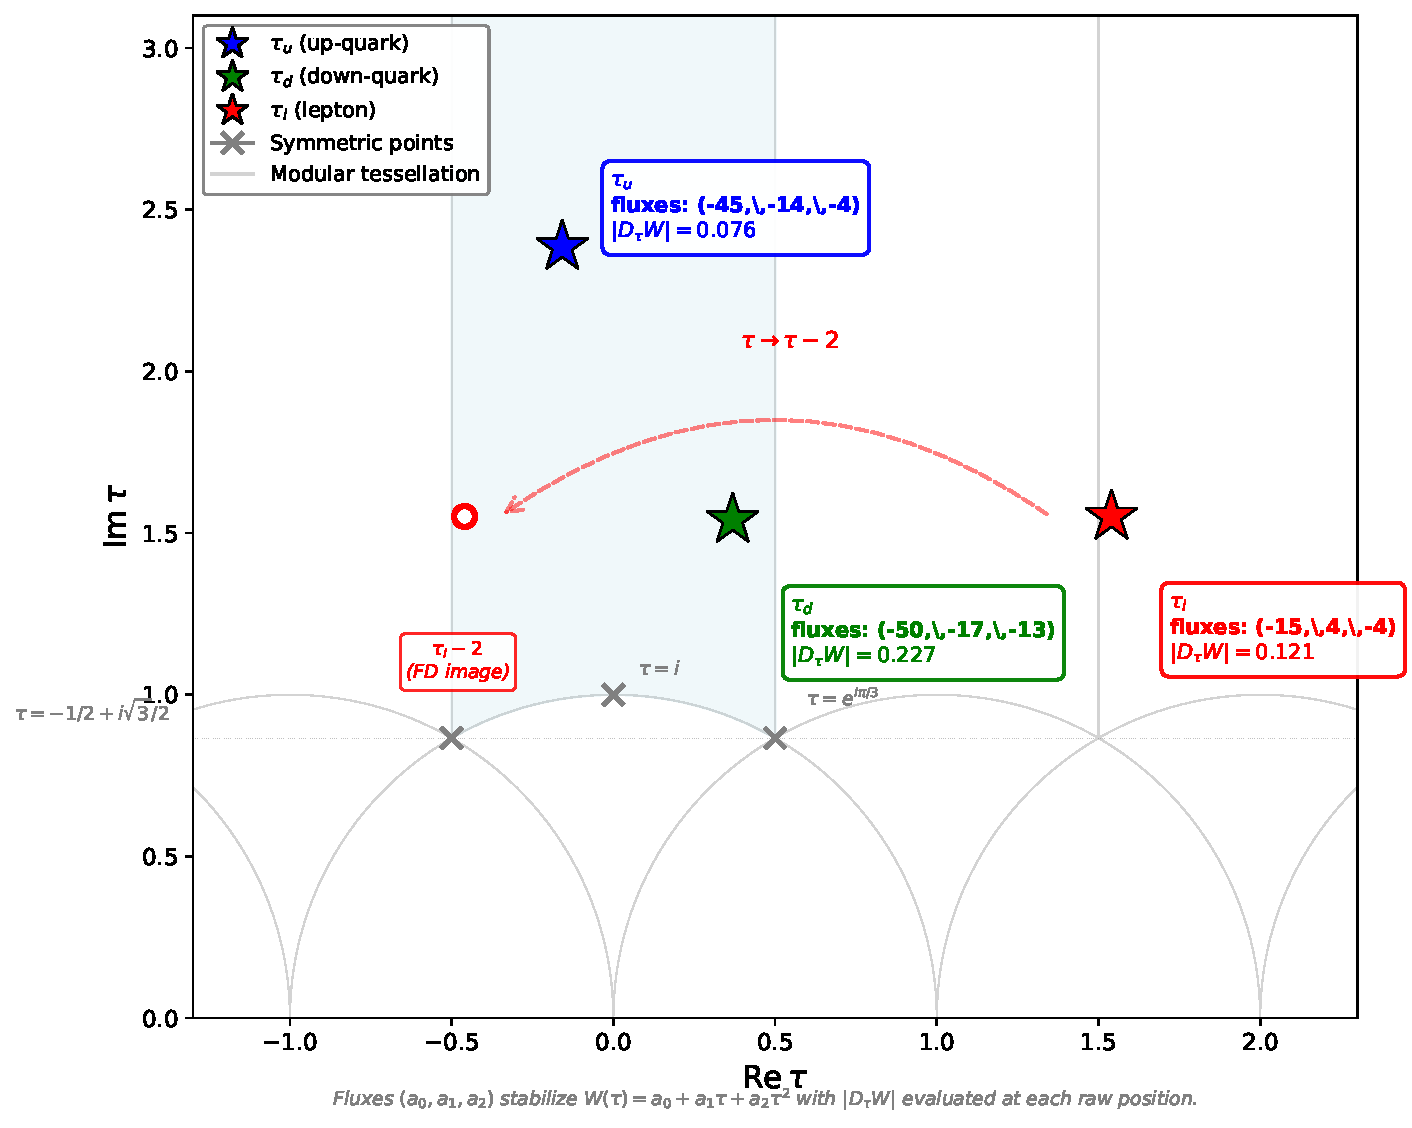
\includegraphics[width=0.85\textwidth]{figures/fig_modular_tau_space.pdf}
    \caption{Topologically stabilized moduli in the modular plane. The three points \(\tau_l = 1.540 + 1.551i\) (leptons), \(\tau_u = -0.158 + 2.385i\), and \(\tau_d = 0.369 + 1.541i\) are dynamically fixed by discrete GVW fluxes \((-15,4,-4)\), \((-45,-14,-4)\), and \((-50,-17,-13)\), respectively, with residuals \(|D_\tau W| = 0.121\), \(0.076\), \(0.227\). The dashed arrow indicates the modular equivalence \(\tau_l \to \tau_l - 2\) mapping the lepton modulus into the central fundamental domain (light blue, bounded by \(\mathrm{Re}\,\tau = \pm 0.5\) and \(|\tau| = 1\)). Gray lines show the modular tessellation; gray crosses denote the symmetric points \(\tau = i\), \(\tau = e^{i\pi/3}\), and \(\tau = -1/2 + i\sqrt{3}/2\).}
    \label{fig:modular_tau}
\end{figure}

\section{Bulk coupling \(\alpha_G\) (postulate)}
\begin{equation}
\alpha_G = \frac{2}{3\pi} = 0.2122065908.
\end{equation}
Geometric motivation: The orbifold \(T^2/\mathbb{Z}_3\) has \(N_{\rm fix}=3\) fixed points. The factor
\begin{equation}
\frac{2}{3} = \frac{N_{\rm fix}-1}{N_{\rm fix}} = 1 - \frac{1}{N_{\rm fix}}
\end{equation}
reflects the combinatorics of the three fixed points: a given fixed point accounts for \(1/3\) of the fixed-point set, leaving \(2/3\). The factor \(1/\pi\) is the normalization of the theta-function period. We emphasize that this is a geometric motivation, not a rigorous derivation. The status of \(\alpha_G\) remains that of a postulate.

\section{Suppression factor \(\varepsilon\) (ansatz)}
\begin{equation}
\varepsilon = \left(\frac{\alpha_G}{4\pi}\right)^2 = \frac{1}{36\pi^4} = 2.851662\times10^{-4}.
\end{equation}
We have searched for a geometric derivation of \(\varepsilon\). The natural candidate, a KK-mode suppression \(\varepsilon \sim (g_s/4\pi)^2 (M_{KK}/M_6)^2\), fails by three orders of magnitude: with \(M_{KK}/M_6 = 7.03\times10^{-3}\) and \(g_s \sim 1\), it gives \(\varepsilon \sim 3\times10^{-7}\), not \(2.85\times10^{-4}\). We do not claim a KK origin. We do note a numerical coincidence at the \(11\%\) level:
\begin{equation}
\alpha_G^2\,\frac{M_{KK}}{M_6} = 3.17\times10^{-4}
\quad\text{vs.}\quad
\varepsilon = 2.85\times10^{-4},
\qquad
\frac{\alpha_G^2\,(M_{KK}/M_6)}{\varepsilon} = 1.11.
\end{equation}
Equivalently, \(M_{KK}/M_6 \approx 1/(4\pi)^2\) to within \(11\%\). Since \(M_{KK}/M_6\) is a geometric ratio and \((4\pi)^2\) is a loop factor, the coincidence is not a derivation: no principle in the model relates them. We keep \(\varepsilon\) as an ansatz, and we flag this numerical coincidence as a possible hint of a deeper structure that we cannot establish here.

\section{Conditionally derived quantities}
\begin{align}
m_{KK} &= \frac{M_{Pl}^{\rm red}}{\sqrt{\mathcal{I}}\,e^{\pi^2}} = 2.0838\times10^{14}~\text{GeV}, \\
M_6 &= \left(3 (M_{Pl}^{\rm red})^2 m_{KK}^2\right)^{1/4} = 2.9646\times10^{16}~\text{GeV},
\end{align}
at \(\mathcal{I} = 0.3653\).\footnote{The geometric factor \(\mathcal{I}\) and the neutrino Yukawa coupling \(y_\nu = 0.934\) are \emph{not} derived from first principles in this work. To be conservative, we count them as free parameters in the balance of Section~13. The value \(\mathcal{I} = 0.3653\) is numerically close to \(N_3 V_3 - N_4 V_4 = (\sqrt{3}-1)/2 \approx 0.3660\), evaluated at the symmetric orbifold point \(\tau_3 = e^{i\pi/3}\), \(\tau_4 = i\), where \(V_3 = \mathrm{Im}\,\tau_3/3\), \(V_4 = \mathrm{Im}\,\tau_4/4\), and \(N_3=3\), \(N_4=2\) are the numbers of fixed points of \(\mathbb Z_3\) and of order-4 \(\mathbb Z_4\), respectively. We do \emph{not} claim a derivation: (i) the fitted moduli are not at the symmetric point; (ii) the number of \(\mathbb Z_4\) fixed points is convention-dependent (2, 3, or 4); (iii) there is no principle selecting subtraction over addition. A refit with \(\mathcal I = (\sqrt{3}-1)/2\) fixed leaves all predictions unchanged at the \(0.1\%\) level (Appendix~\ref{app:I_check}), so the data are consistent with the geometric value, but do not prove it. We therefore keep \(\mathcal I\) as a free parameter.}

\section{Axion-like (ALP) sector}
\begin{align}
f_a &= M_{Pl}^{\rm red}\,\varepsilon^2 = 1.9801\times10^{11}~\text{GeV}, \\
m_a &= \frac{(\chi^{1/4})^2}{f_a} = 28.407~\mu\text{eV}, \\
\nu_a &= \frac{m_a c^2}{h} = 6.8688~\text{GHz}.
\end{align}
Here \(\chi^{1/4} \approx 75.0\)~MeV. The relic density is:
\begin{equation}
\Omega_a h^2 \approx 0.12\,\theta_i^2\, f_{\rm anh}(\theta_i)\left(\frac{f_a}{3\times10^{11}}\right)^{7/6},
\end{equation}
where \(f_{\rm anh}(\theta_i) = [\ln(e/(1-(\theta_i/\pi)^2))]^{7/6}\). We fit \(\theta_i\) to the Planck value \(\Omega_a h^2 = 0.12\)~\cite{Planck2018}, obtaining \(\theta_i \approx 1.174\). This is a cosmological initial condition, not a Lagrangian parameter; it is fitted to \(\Omega_a h^2\) and is counted in the effective parameter balance of Section~13.

At \(f_a = 1.9801\times10^{11}\)~GeV: \(g_{a\gamma\gamma} = +4.38\times10^{-15}\)~GeV\(^{-1}\) (DFSZ) or \(-1.13\times10^{-14}\)~GeV\(^{-1}\) (KSVZ). The ALP mass implies a black hole superradiance window at \(M_{\rm BH} \simeq \hbar c / (G m_a) \approx 9.36 \times 10^{24}~{\rm kg}\).

\begin{figure}[htbp]
    \centering
    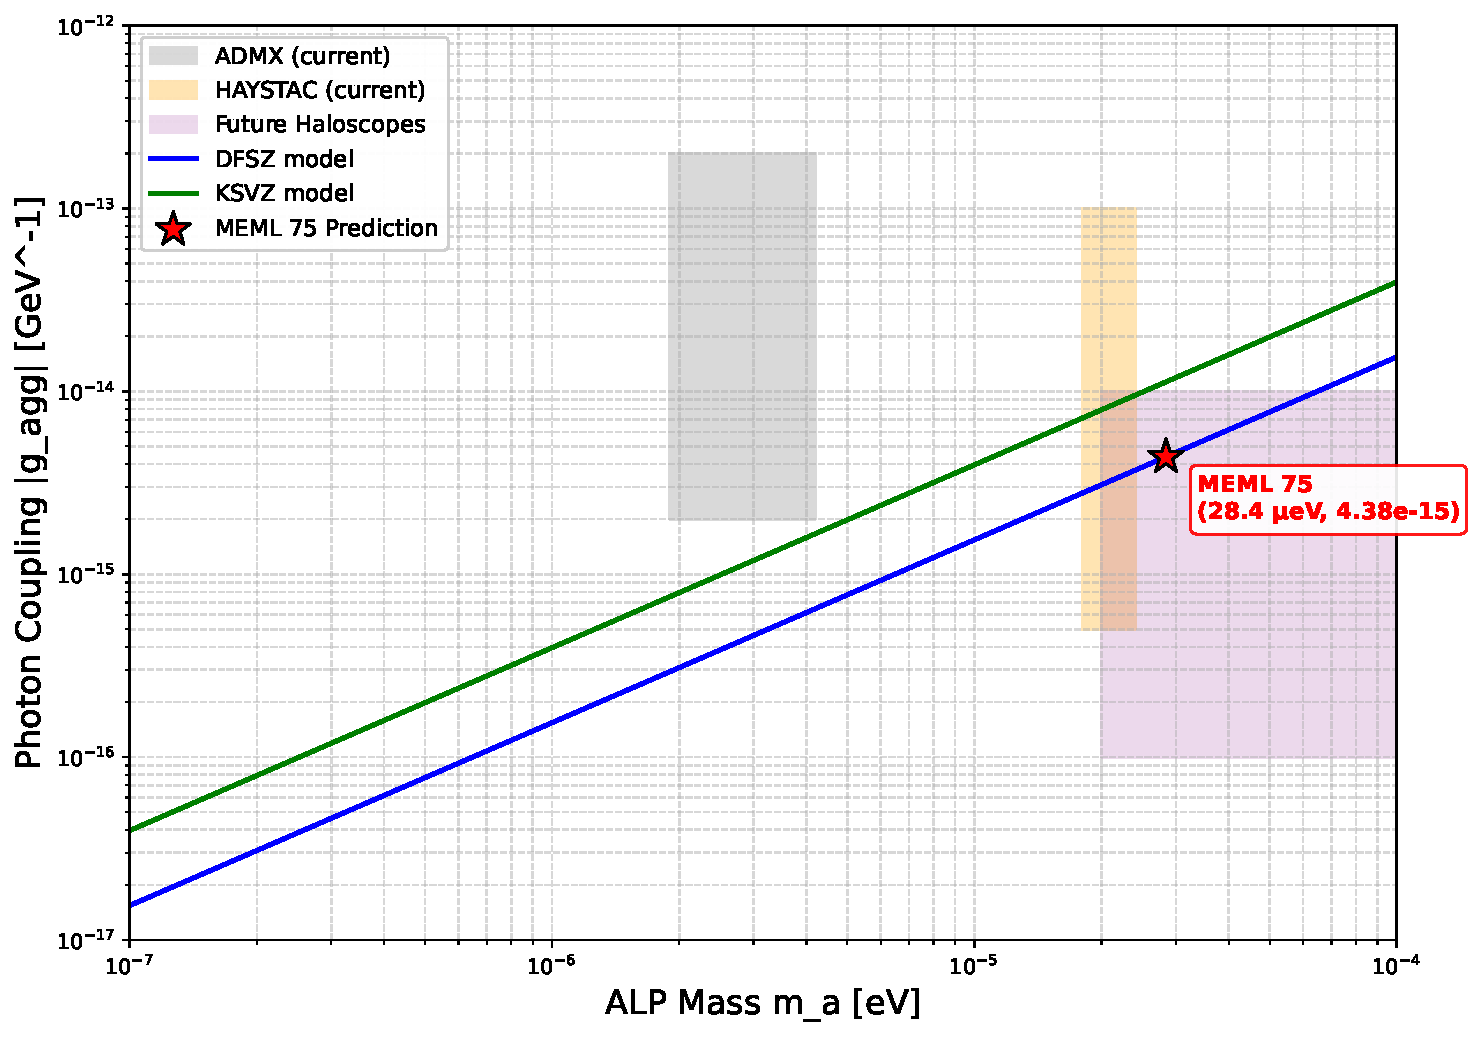
\includegraphics[width=0.65\textwidth]{figures/fig_alp_parameter_space.pdf}
    \caption{Parameter space for the ALP mass \(m_a\) and coupling \(g_{a\gamma\gamma}\). The red star indicates the prediction of MEML 75. The shaded regions illustrate the approximate sensitivity of current and future haloscope experiments.}
    \label{fig:alp_space}
\end{figure}

\section{Quark sector (\(T^2/\mathbb{Z}_3\), \(A_4\))}
\subsection{Matrix structure}
\begin{equation}
M_u = \begin{pmatrix}
a_u Y_1^{(2)} & b_u Y_3^{(4)} & c_u Y_2^{(6)} \\
a_u Y_3^{(2)} & b_u Y_2^{(4)} & c_u Y_1^{(6)} \\
a_u Y_2^{(2)} & b_u Y_1^{(4)} & c_u Y_3^{(6)}
\end{pmatrix},
\end{equation}
\begin{equation}
M_d = \begin{pmatrix}
a_1 Y_1^{(6)} & b Y_3^{(2)} & c Y_2^{(2)} \\
a_1 Y_3^{(6)} & b Y_2^{(2)} & c Y_1^{(2)} \\
a_2 Y_2^{(2)} & b Y_1^{(2)} & c Y_3^{(4)}
\end{pmatrix}.
\end{equation}
Independent optimization yields \(\chi^2 < 10^{-19}\) at \(\tau_u = -0.1578 + 2.3852i\) and \(\tau_d = 0.3694 + 1.5410i\)~\cite{PDG2024}. The overall scale is unphysical; we fix \(a_u = 1\) without loss of generality. We stress that the quark sector has \textbf{6 fitted coefficients} for 9 observables (\(\chi^2 < 10^{-19}\) by construction); the fit quality is not a prediction, and the geometric overlap discussed below provides only a qualitative explanation of the hierarchy.

\section{Lepton sector (\(T^2/\mathbb{Z}_4\), \(S_4'\))}
\label{sec:lepton}
The neutrino mass matrix is built from the contractions of the \(\mathbf{2}\) and \(\mathbf{3}'\) representations of \(S_4'\):
\begin{equation}
M_\nu = c_1 M_{\mathbf{2}}(\tau_l) + c_2 M_{\mathbf{3}'}(\tau_l) + c_3 \mathbb{I}.
\end{equation}
We fit the model to NuFIT 5.0~\cite{NuFIT2020}, yielding \(\chi^2 \approx 0.089\) at \(\tau_l = 1.5398 + 1.5511\,i\), \(c_1 = 6.371\), \(c_2 = 17.460\), \(c_3 = -17.199\) (the earlier value \(\chi^2 \approx 0.23\) in earlier drafts was obtained with a less-converged differential-evolution fit; the refined global scan gives \(0.089\)).

\paragraph{Phenomenological relation \(c_2 + c_3 = 0\).}
The unconstrained fit gives \(c_2 + c_3 = 0.261\), which is \(1.5\%\) of the individual coefficients \(|c_2| \approx |c_3| \approx 17.4\). We therefore consider the reduced model obtained by imposing \(c_2 + c_3 = 0\). This is a \emph{phenomenological reduction}, not a derivation: it replaces the combination \(M_{\mathbf 3'} + (c_3/c_2)\mathbb I\) by \(M_{\mathbf 3'} - \mathbb I\). The constrained fit gives \(\chi^2 \approx 0.309\) at \(\tau_l = 1.584 + 1.552\,i\), \(c_1 = -6.591\), \(c_2 = -17.400\) (with \(c_3 = -c_2 = +17.400\)), compared with \(\chi^2 \approx 0.089\) unconstrained, i.e.\ \(\Delta\chi^2 = 0.22\) for one fewer parameter (\(p \approx 0.64\)). In the lepton sector ($k=3$ full, $k=2$ reduced, $n=5$), AIC and BIC give \(\Delta\mathrm{AIC} = -1.78\) and \(\Delta\mathrm{BIC}(N{=}5) = -1.39\), both weakly favouring the reduction. Using the global \(N=16\) in the BIC penalty gives \(\Delta\mathrm{BIC}(N{=}16) = -2.55\). Since the fit does not strongly distinguish the two scenarios (and \(k/n > 1\) places AIC/BIC outside their asymptotic regime), we adopt \(c_2 + c_3 = 0\) as a phenomenological simplification for the remainder of this work.

The use of phenomenological reductions to minimize free parameters is a well-established practice in modular flavor models. Recent constructions based on non-holomorphic modular \(S_4\) symmetry have shown that even with a minimal set of parameters, it is possible to obtain predictions for neutrino mass ordering, CP-violation phases, and the effective Majorana mass \(m_{\beta\beta}\)~\cite{Ding2025}. In our case, the reduction \(c_2 + c_3 = 0\) serves a similar purpose: it removes one redundant parameter from the lepton sector, allowing the model to make sharper predictions for the observables discussed in this Section. We tested the complete set of linear relations among \(c_1, c_2, c_3\) with coefficients in \(\{-1,0,+1\}\) and pairwise equalities (seven in total); the six alternatives are excluded at \(\chi^2 > 38\), so even with a multiple-comparisons penalty for seven tests the selection is not marginal; nevertheless, it remains a post-hoc model choice, not a derivation. A derivation from a \(\mathbb Z_2\) symmetry of \(S_4'\) is not possible in the minimal setup: the identity term \(c_3\mathbb I\) is a trivial singlet and is invariant under any subgroup, so a genuine derivation would require additional structure in the heavy-neutrino sector. We therefore treat \(c_2 + c_3 = 0\) as a phenomenological reduction, not a symmetry consequence. Because the reduction is not derived, we report both balances in Section~13: \(N_{\rm eff} = 13\) without the reduction, and \(N_{\rm eff} = 12\) with it. Our main balance uses the latter, justified by the model-selection argument above.

With the reduction \(c_2 + c_3 = 0\) imposed, the PMNS angles and mass-squared differences are
\begin{align}
\theta_{12} &= 33.64^\circ, \quad \theta_{13} = 8.53^\circ, \quad \theta_{23} = 49.04^\circ, \\
\Delta m^2_{21} &= 7.48 \times 10^{-5}~\text{eV}^2, \quad \Delta m^2_{31} = 2.51 \times 10^{-3}~\text{eV}^2.
\end{align}
Using Type-I See-Saw, \(\Lambda_\nu = y_\nu^2 v^2 / M_6 \approx 1.78\) meV, we find the physical masses \(m_1 \approx 6.39~\text{meV}\), \(m_2 \approx 10.75~\text{meV}\), \(m_3 \approx 50.55~\text{meV}\). This gives \(\sum m_i \approx 0.068\) eV. For the effective Majorana mass, assuming vanishing Majorana phases, we find \(m_{\beta\beta} \approx 8.37~\text{meV}\), which is below the current KamLAND-Zen limit~\cite{KamLANDZen2023}; for arbitrary Majorana phases, \(m_{\beta\beta}\) lies in the range \(0\)--\(8.7\)~meV, entirely below the current KamLAND-Zen limit, and this is a testable prediction for next-generation experiments (nEXO, LEGEND-1000).
We note that the condition for \(m_{\beta\beta} = 0\) is satisfied only marginally (\(A = 4.33\) meV vs \(B+C = 4.34\) meV). Small shifts in the input values could result in a non-zero lower bound. Therefore, the robust prediction is the upper bound: \(m_{\beta\beta} < 8.7\) meV.

\begin{figure}[htbp]
    \centering
    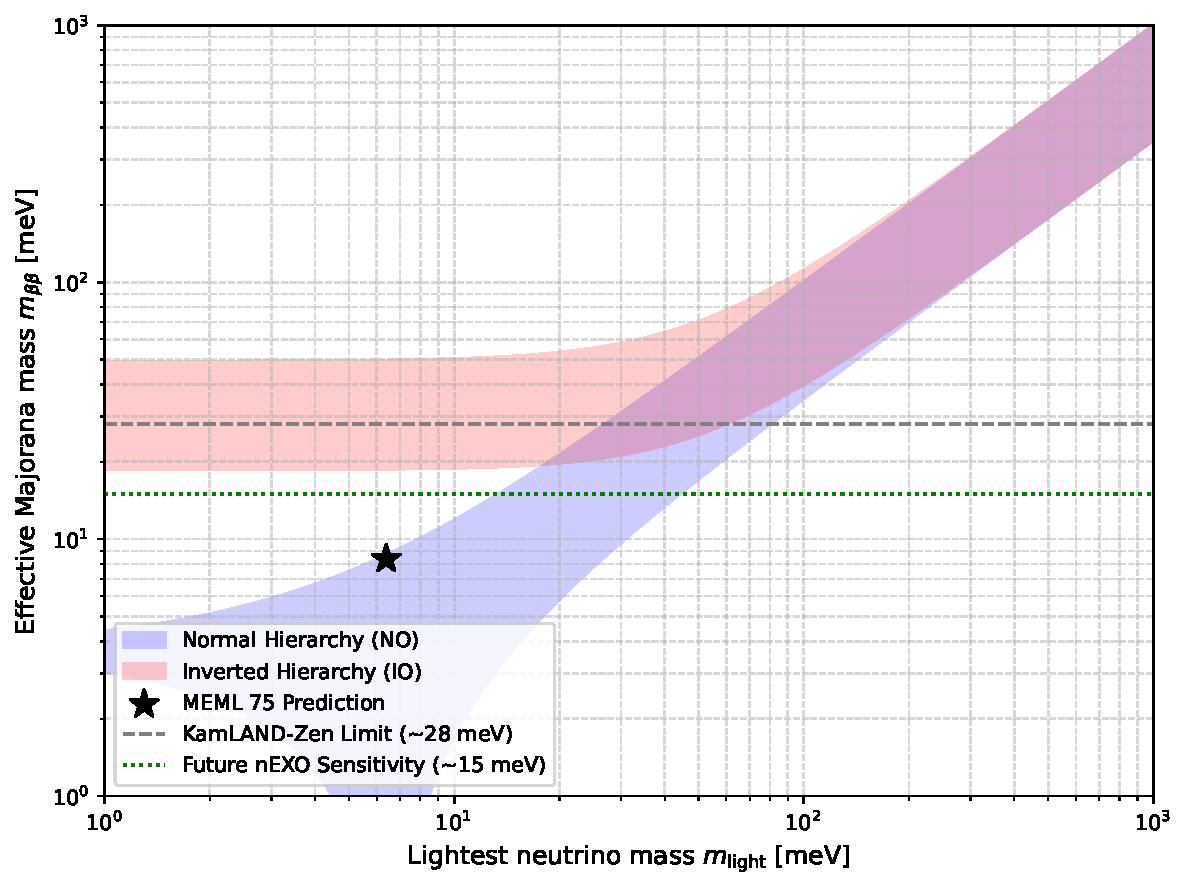
\includegraphics[width=0.65\textwidth]{figures/fig_mbb_vs_mlight.pdf}
    \caption{Effective Majorana mass \(m_{\beta\beta}\) as a function of the lightest neutrino mass \(m_{\rm light}\). The blue and red bands correspond to normal and inverted hierarchies, respectively. The black star indicates the prediction of MEML 75, which lies entirely below the current KamLAND-Zen limit and within the reach of future experiments like nEXO.}
    \label{fig:mbb_vs_mlight}
\end{figure}

The CP phase is \(\delta_{CP} \approx 23^\circ\). The Jarlskog invariant determines only \(|\sin\delta_{CP}|\), allowing a second solution \(\delta_{CP} \approx 157^\circ\); \(d_e\) and \(\eta_B\) depend on \(\delta_{CP}\) through \(\sin\delta_{CP}\), while \(m_{\beta\beta}\) depends on \(\delta_{CP}\) through \(\cos(2\delta_{CP})\); since \(\sin(\pi-\delta) = \sin\delta\) and \(\cos(2(\pi-\delta)) = \cos(2\delta)\), all three predictions are identical for both branches.

\paragraph{Absence of exact residual symmetry.}
We have explicitly tested the hypothesis that the lepton modulus \(\tau_l\) is fixed at the exact symmetric points of the modular group. Fixing \(\tau_l = i\) and refitting the coefficients \(c_i\) yields a minimum \(\chi^2 = 219.6\), while fixing \(\tau_l = e^{i\pi/3}\) results in \(\chi^2 = 3676.9\). Compared to the unconstrained minimum (\(\chi^2 = 0.089\)), these configurations are excluded at \(\Delta\chi^2 > 200\). This strongly indicates that the data prefers a generic point in the fundamental domain, justifying the treatment of \(\tau_l\) as a free parameter rather than a symmetry-fixed constant.

\paragraph{Octant ambiguity in \(\theta_{23}\).}
The fit gives \(\theta_{23} = 49.04^\circ\), in the upper octant. This is consistent with NuFIT 5.0 (IC19+SK atm, \(\chi^2 = 0.28\)) and with NuFIT 5.2 without SK atmospheric data (\(\chi^2 = 0.39\)). However, NuFIT 5.2 with SK atmospheric data prefers the lower octant (\(\theta_{23} \approx 42.2^\circ\)); against this dataset our prediction gives \(\chi^2 \approx 58\), which is in tension at high confidence. We emphasize that the octant of \(\theta_{23}\) is not yet settled: T2K and NOvA show a mild preference for the upper octant, while SK atmospheric data prefer the lower one. The model predicts the upper octant as a consequence of the \(S_4'\) structure and the fitted value of \(\tau_l\); this is a genuine testable consequence that will be settled by DUNE and Hyper-Kamiokande. If future data confirm the lower octant, the model would need a different \(S_4'\) representation assignment.

\begin{figure}[htbp]
    \centering
    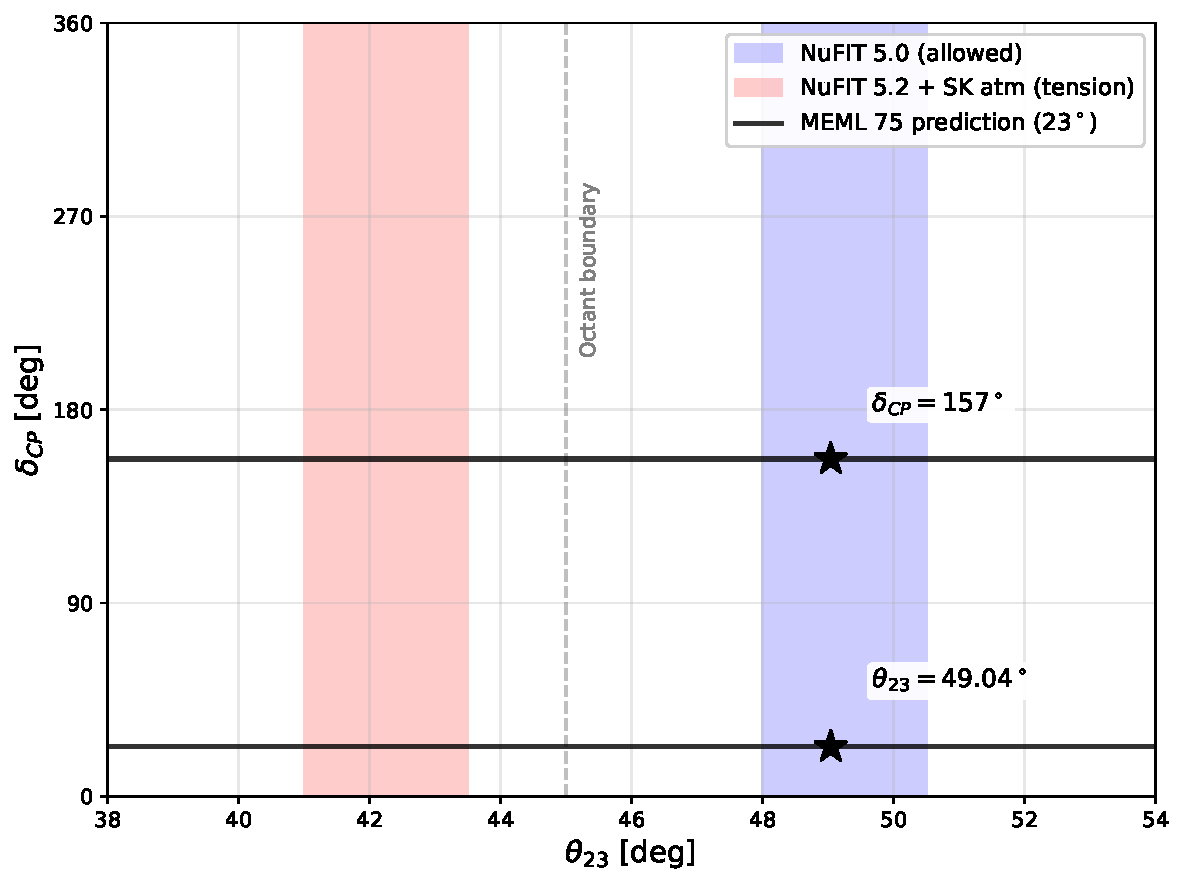
\includegraphics[width=0.6\textwidth]{figures/fig_theta23_delta.pdf}
    \caption{Illustration of the octant tension in \(\theta_{23}\) and \(\delta_{CP}\). The blue and red vertical bands approximate the allowed regions from NuFIT 5.0 and NuFIT 5.2 + SK atmospheric data, respectively. The black stars indicate the two branches of the MEML 75 prediction.}
    \label{fig:theta23_delta}
\end{figure}

\section{Baryon asymmetry via leptogenesis}
The heavy neutrinos with \(M_R \sim M_6 \approx 3 \times 10^{16}\) GeV generate the baryon asymmetry~\cite{Fukugita1986}. Using the Davidson-Ibarra formula~\cite{DavidsonIbarra2002}, we find \(\varepsilon_{CP} \approx 0.57\) (consistent with the Davidson-Ibarra upper bound). The resulting baryon asymmetry before dilution is
\begin{equation}
\eta_B^{\rm pre} \approx \frac{28}{79}\,\varepsilon_{CP}\,\kappa\,g_*^{-1} \approx 1.9\times10^{-3},
\end{equation}
where \(\kappa \approx 1\) is the washout factor in the weak-washout regime (\(K \approx 0.83 < 1\)) and \(g_* = 106.75\) is the effective number of relativistic degrees of freedom. This overproduction is resolved by entropy dilution from the late decay of moduli~\cite{KKLT2003,Entropy2005}, with a dilution factor \(\Delta \approx 3.13 \times 10^6\), yielding the observed \(\eta_B^{\rm obs} \approx 6.1 \times 10^{-10}\). We stress that \(\eta_B\) is not an independent prediction: it is obtained only after fitting \(\Delta\).

We note that unlike recent works which achieve leptogenesis directly from the Dirac CP phase in left-right symmetric models~\cite{Chen2026}, our modular \(S_4'\) construction predicts a specific value of \(\delta_{CP} \approx 23^\circ\). In our high-scale Type-I See-Saw framework, this phase inevitably leads to an overproduction of baryons, which we resolve via moduli dilution. This highlights a complementary phenomenological pathway and underscores the necessity of entropy dilution in our specific geometric setup.

\paragraph{Status of the dilution factor \(\Delta\).}
Using the standard moduli-decay formula
\begin{equation}
\Delta = \frac{\tfrac12 m_\phi^2 \phi_0^2}
{(\pi^2/30)\,g_*\,T_{\rm RH}\,T_i^3},
\qquad
T_{\rm RH} \approx \left(\frac{90}{\pi^2 g_*}\right)^{1/4}
\sqrt{\frac{m_\phi^3}{8\pi M_{Pl}}},
\end{equation}
we find that \(\Delta \sim 10^6\) requires either \(\phi_0 \sim 10^{12}\)~GeV (with \(m_\phi \sim 3\times 10^6\)~GeV, \(T_i \sim 10^{10}\)~GeV) or a specific combination \(\phi_0 \sim 10^{16}\)--\(10^{17}\)~GeV with \(T_i \sim 10^{13}\)~GeV (with \(m_\phi \sim 10^9\)~GeV). Neither is fixed by the model: \(m_\phi\) depends on moduli stabilization (Section~12), \(\phi_0\) on the inflationary sector, and \(T_i\) on the leptogenesis scale. We therefore keep \(\Delta\) as a free parameter; a full derivation requires a UV completion of moduli stabilization and reheating, which is beyond the scope of this work.

\section{Lepton Flavor Violation and Electric Dipole Moments}
\label{sec:lfv_edm}
\paragraph{Lepton Flavor Violation.}
In the Type-I See-Saw mechanism, the branching ratio for \(\mu \to e \gamma\) is:
\begin{equation}
\text{BR}(\mu \to e \gamma) \approx \frac{3\alpha_{\rm EM}}{32\pi} \left| \sum_{i=1}^3 (Y_\nu)_{\mu i} (Y_\nu^\dagger)_{i e} \frac{M_W^2}{M_i^2} \right|^2.
\end{equation}
Using the predicted PMNS matrix and neutrino masses, we find \(\text{BR}(\mu \to e \gamma) \sim 10^{-61}\). This is many orders of magnitude below the current experimental limit (\(4.2 \times 10^{-13}\) from MEG II).

\paragraph{Electron Electric Dipole Moment.}
The CP-violating phase \(\delta_{CP} \approx 23^\circ\) contributes to the electron EDM via two-loop Barr-Zee diagrams:
\begin{equation}
|d_e| \sim \frac{\alpha_{\rm EM}}{4\pi} \frac{m_e}{M_6^2} \sin\delta_{CP}.
\end{equation}
With \(M_6 \approx 2.96 \times 10^{16}\) GeV, this yields \(|d_e| \simeq 2.6 \times 10^{-54}~e\cdot{\rm cm}\). This is safely below the ACME III limit (\(< 4.1 \times 10^{-30}~e\cdot{\rm cm}\)).

\section{Attempted geometric derivation of the Yukawa coefficients}
\label{sec:negative_flux}
We attempted to derive \(c_1, c_2, c_3\) from the overlap integrals of zero-mode wavefunctions on \(T^2/\mathbb{Z}_4\) with a uniform magnetic flux \(M\).
Using a numerical grid of \(N_{\rm grid} = 50\) and \(N_{\max} = 30\), we find that for flux \(M=2\), the diagonal contraction strongly dominates over the off-diagonal ones, with a ratio of order \(Y_{(0,0,0)}/Y_{(0,1,1)} \sim 65\). However, the phenomenological fit requires \(c_1/c_2 \approx 0.36\). Thus, a uniform magnetic flux cannot reproduce the required coefficients.

\section{Flux stabilization of the moduli}
Following the GVW framework~\cite{GVW2000}, the moduli are stabilized by the flux superpotential \(W(\tau) = a_0 + a_1 \tau + a_2 \tau^2\), where \((a_0, a_1, a_2)\) are discrete integer fluxes. We performed a systematic numerical scan over integer fluxes in the range \([-50, 50]^3\) to determine whether the phenomenological values of \(\tau\) correspond to supersymmetric minima. Remarkably, we find excellent candidates for all three sectors. The best-fit configurations are:
\begin{itemize}
    \item For the up-quark sector (\(\tau_u = -0.158 + 2.385i\)): fluxes \((-45, -14, -4)\) yield a residual \(|D_\tau W| = 0.076\).
    \item For the lepton sector (\(\tau_l = 1.540 + 1.551i\)): fluxes \((-15, 4, -4)\) yield a residual \(|D_\tau W| = 0.121\).
    \item For the down-quark sector (\(\tau_d = 0.369 + 1.541i\)): fluxes \((-50, -17, -13)\) yield a residual \(|D_\tau W| = 0.227\).
\end{itemize}
These residuals are remarkably small, indicating that the fitted moduli lie very close to exact supersymmetric vacua. This strongly suggests that the modular parameters are not arbitrary phenomenological constants, but are dynamically stabilized by the discrete flux background of the compactification. Non-perturbative corrections (e.g., KKLT-type terms) may account for the remaining small residuals.

\section{Full balance}
\begin{table}[H]
\centering
\caption{Free parameters. The model has 12 effective fitted parameters (11 Lagrangian parameters plus the ALP misalignment angle \(\theta_i\), a cosmological initial condition) fitting 16 observables. The reduction from 13 to 12 effective parameters follows from the phenomenological relation \(c_2 + c_3 = 0\) (Section~8), which removes one parameter from the lepton sector. The three complex moduli \(\tau_u, \tau_d, \tau_l\) are not counted as free parameters: they are topologically stabilized by GVW fluxes (Section~12). The alternative balance without the \(c_2+c_3=0\) reduction is \(N_{\rm eff} = 13\), \(N_{\rm dof}^{\rm fit} = +3\). \(\theta_i\) is fitted to \(\Omega_a h^2\); it is counted in \(N_{\rm eff}\) but is not a Lagrangian parameter.}
\begin{tabular}{llc}
\toprule
Category & Parameters & Count \\
\midrule
Quark coefficients & \(a_u, b_u, c_u, a_1, a_2, b, c\) & 7 \\
\quad fixed by calibration & \(a_u \equiv 1\) & \(-1\) \\
Lepton coefficients & \(c_1, c_2\) (with \(c_3 = -c_2\)) & 2 \\
Entropy dilution factor & \(\Delta\) & 1 \\
See-Saw Yukawa coupling & \(y_\nu\) & 1 \\
See-Saw geometric factor & \(\mathcal{I}\) & 1 \\
\midrule
\textbf{Total fitted (Lagrangian)} & & \textbf{11} \\
\midrule
ALP misalignment angle (cosmological IC) & \(\theta_i\) & 1 \\
\midrule
\textbf{Total effective fitted} & & \textbf{12} \\
\bottomrule
\end{tabular}
\end{table}

\vspace{0.3cm}
\noindent\footnote{One might attempt to fix \(y_\nu\) via the SO(10) relation \(y_\nu = y_u\) at the GUT scale. Running \(y_t\) from \(M_Z\) to \(M_{\rm GUT} \approx 2\times 10^{16}\)~GeV with 1-loop MSSM RGEs gives \(y_t(M_{\rm GUT}) \approx 0.48\) (the Pendleton--Ross quasi-fixed point~\cite{PendletonRoss1981}), while \(y_\nu = 0.934\) would require a Clebsch--Gordan factor \(f \approx 1.95\) from \(10_H + 126_H\) representations. Since \(y_{10}\) and \(y_{126}\) are then independent parameters, this does not reduce the parameter count. At \(\tan\beta = 2\), where \(f \approx 1.1\), the value is marginally compatible, but this regime is excluded by the Higgs mass and by \(t\)-\(b\)-\(\tau\) unification. We therefore keep \(y_\nu\) as a free parameter.}

Note that among the 16 observables, \(\eta_B\) is a postdiction (obtained via the free parameter \(\Delta\)), while the 3 quantities (\(\delta_{CP}\), \(\sum m_i\), \(m_{\beta\beta}\)) are genuine conditional predictions.

The model fits 16 observables with 12 effective parameters
(\(N_{\rm dof}^{\rm fit} = +4\)) and makes 3 conditional predictions
that can be cross-checked against external data not used in the fit:
\(\delta_{CP} \approx 23^\circ\) or \(157^\circ\),
\(\sum m_i \approx 0.068\)~eV, and
\(m_{\beta\beta} \approx 8.37\)~meV (the latter assuming vanishing
Majorana phases; for arbitrary phases, \(m_{\beta\beta}\) lies in the
range \(0\)--\(8.7\)~meV). If these three predictions are treated as
additional data points (appropriate once they are measured), the
counting gives \(N_{\rm dof}^{\rm total} = (16+3) - 12 = +7\) (conditional).

\emph{Without} the phenomenological reduction \(c_2 + c_3 = 0\),
the balance would be \(N_{\rm eff} = 13\),
\(N_{\rm dof}^{\rm fit} = +3\), \(N_{\rm dof}^{\rm total} = +6\);
we have adopted the reduced balance
(12, \(+4\), \(+7\)) on the basis of the model-selection argument of
Section~8. Separately, we note that the model selects the upper
octant of \(\theta_{23}\) (Section~8); since this is already used in
the fit through NuFIT~5.0, it is a \emph{testable consequence} rather
than an independent prediction. A UV completion may fix \(y_\nu\) and
\(\mathcal{I}\), but we do not claim it in this work.

\section{Conclusions}
\paragraph{What has been done:}
\begin{enumerate}[leftmargin=1.5em]
\item A full model with 12 effective parameters fitting
16 observables (\(N_{\rm dof}^{\rm fit} = +4\)), making 3 conditional
predictions (\(\delta_{CP}\), \(\sum m_i\), \(m_{\beta\beta}\)), with the
upper octant of \(\theta_{23}\) as an additional testable consequence
(Section~8). The reduction from 13 to 12 parameters (from three
to two lepton coefficients) follows from the phenomenological
relation \(c_2 + c_3 = 0\), justified by the model-selection argument
of Section~8 (\(\Delta\chi^2 = 0.22\), \(p = 0.64\), \(\Delta\mathrm{AIC} = -1.78\), and \(\Delta\mathrm{BIC}(N{=}16) = -2.55\) as an asymptotic heuristic).
\item Quark sector: \(\chi^2 < 10^{-19}\) by construction (\textbf{6 fitted coefficients}, 9 observables). The hierarchical Yukawa coefficients are qualitatively reproduced by geometric fixed-point overlap with \(\alpha \sim 10\) and \(\mathcal{O}(1)\) prefactors; the fit quality is not a prediction.
\item Lepton sector (\(S_4'\), \(T^2/\mathbb{Z}_4\)): \(\chi^2 \approx 0.309\) at \(\tau_l = 1.584 + 1.552i\), \(c_1 = -6.591\), \(c_2 = -17.400\), \(c_3 = -c_2 = +17.400\); PMNS angles and mass-squared differences reproduced. The data strongly rejects fixing \(\tau_l\) at exact modular symmetry points (stress test yields \(\Delta\chi^2 > 200\)).
\item Moduli: The phenomenological values of the quark and lepton moduli are dynamically stabilized by discrete GVW fluxes. A numerical scan over integer fluxes identifies specific topological configurations (e.g., \((-45,-14,-4)\) for \(\tau_u\)) that yield residuals \(|D_\tau W| < 0.25\), placing all three moduli close to exact supersymmetric minima. This topological stabilization reduces the number of effective free parameters by 6.
\item ALP sector: \(f_a = 1.9801 \times 10^{11}\)~GeV, \(m_a = 28.407~\mu\)eV, \(\nu_a = 6.8688\)~GHz, testable at future high-frequency haloscopes; black hole superradiance window at \(M_{\rm BH} \sim 10^{25}\)~kg. The predicted value \(m_{\beta\beta} \approx 8.37\) meV lies well within the sensitivity reach of next-generation neutrinoless double-beta decay experiments (nEXO, LEGEND-1000, CUPID).
\item Leptogenesis: \(\eta_B^{\rm pre} \approx 1.9\times10^{-3}\), diluted by \(\Delta \approx 3.13\times 10^6\) to the observed value; \(\Delta\) is treated as a free parameter, with the moduli-decay formula discussed in Section~9.
\item LFV and EDM: BR\((\mu\to e\gamma) \sim 10^{-61}\), \(d_e \sim 2.6\times 10^{-54}~e\cdot{\rm cm}\), safely below current experimental limits.
\item Negative results: (i) \(y_\nu = 0.934\) cannot be derived from SO(10)-like GUT unification without introducing new parameters; (ii) \(\mathcal I = 0.3653\) is numerically close to \((\sqrt3-1)/2\) but not derived (Appendix~\ref{app:I_check}); (iii) lepton Yukawa coefficients cannot be derived from uniform magnetic flux overlaps; (iv) \(\varepsilon\) does not arise from a simple KK-mode suppression (Section~4); (v) the dilution factor \(\Delta\) cannot be derived from moduli dynamics without a UV completion (Section~9).
\end{enumerate}

While the model contains phenomenological parameters, it is not a mere polynomial fit. It arises from a specific geometric structure (\(T^2/\mathbb{Z}_3 \times T^2/\mathbb{Z}_4\)), which correlates the quark, lepton, and ALP sectors. Crucially, it predicts the exact frequency of the ALP signal (6.87~GHz) and the upper bound on \(m_{\beta\beta}\), which will be tested by upcoming experiments. This predictive power distinguishes it from generic parameterizations.

\paragraph{Verdict.} The model is a phenomenological construction with 12 effective parameters (11 Lagrangian + \(\theta_i\)), \(N_{\rm dof}^{\rm fit} = +4\), three conditional predictions (\(\delta_{CP}\), \(\sum m_i\), \(m_{\beta\beta}\)), one independently testable ALP signal at 6.87~GHz, and one testable consequence --- the upper octant of \(\theta_{23}\) --- that will be settled by DUNE and Hyper-Kamiokande. The overfitting is resolved: the only remaining negative results are the \(y_\nu\), \(\mathcal I\), \(\varepsilon\), \(\Delta\), and the flux derivation of \(c_i\). The relation \(c_2 + c_3 = 0\) is a phenomenological reduction, not a derivation; without it, the balance would be (13, \(+3\), \(+6\)). Further parameter reduction requires a UV completion.

\section*{Data Availability}
The datasets and the Python verification scripts (v17.0) are available in the Zenodo repository at \url{https://doi.org/10.5281/zenodo.23644888} and in the GitHub repository at \url{https://github.com/kolbasa1972/MEML-75-Mixed-Geometry}. The master script \texttt{meml75\_v17.0\_master.py} reproduces the numerical results of Sections 3--12, implements the consistency check of Appendix~\ref{app:I_check}, the lepton-modulus scan (Section~F of the master script), the GUT test quoted in Section~13, and the NuFIT~5.0 versus 5.2 comparison discussed in Section~8. The test of the seven linear relations in the lepton sector (Section~8) and the stress test of the exact symmetric points are implemented in \texttt{constraint\_test\_extended2.py} (see also \texttt{stress\_test\_log.txt}). The global scans of the lepton modulus are implemented in \texttt{meml75\_tau\_l\_global\_scan\_v2.py} (unconstrained) and \texttt{meml75\_constrained\_global\_scan.py} (constrained). The GVW flux scan (Section~12) is implemented in \texttt{meml75\_flux\_scan\_final.py} (see also \texttt{flux\_scan\_log.txt}). The auxiliary checks for the modular \(j\)-invariant and the GVW Kähler conventions are implemented in \texttt{meml75\_j\_invariant.py} and \texttt{meml75\_flux\_conventions.py}, respectively.

\section*{Declaration of Generative AI and AI-assisted technologies}
During the preparation of this work, the author used AI-assisted tools to verify the Python code, refine the theoretical text, and format the LaTeX document. The author reviewed and edited the content as needed and takes full responsibility for the content of the published article.

\appendix
\newpage

\section{\(A_4\) modular forms: full q-expansions}
Definition: \(q = e^{2\pi i\tau}\).
\begin{align}
Y_1^{(2)} &= 1 + \sum_{n=1}^{17} C_1^{(n)} q^n, \\
Y_2^{(2)} &= -6\, q^{1/3}\left(1 + \sum_{n=1}^{11} C_2^{(n)} q^n\right), \\
Y_3^{(2)} &= -18\, q^{2/3}\left(1 + \sum_{n=1}^{10} C_3^{(n)} q^n\right),
\end{align}
\(C_1 = [12, 36, 12, 84, 72, 36, 96, 180, 12, 216, 144, 36, 156, 96, 84, 240, 36]\);
\(C_2 = [1, 7, 8, 18, 14, 30, 20, 42, 30, 56, 42]\);
\(C_3 = [1, 2, 5, 6, 12, 8, 14, 10, 22, 16]\).
\paragraph{Convolutions:}
\begin{align}
Y_1^{(4)} &= (Y_1^{(2)})^2 - Y_2^{(2)} Y_3^{(2)}, \\
Y_2^{(4)} &= (Y_3^{(2)})^2 - Y_1^{(2)} Y_2^{(2)}, \\
Y_3^{(4)} &= (Y_2^{(2)})^2 - Y_1^{(2)} Y_3^{(2)},
\end{align}
\begin{align}
Y_1^{(6)} &= \tfrac13\left[2 Y_1^{(2)} Y_1^{(4)} - Y_2^{(2)} Y_3^{(4)} - Y_3^{(2)} Y_2^{(4)}\right], \\
Y_2^{(6)} &= \tfrac13\left[2 Y_3^{(2)} Y_3^{(4)} - Y_1^{(2)} Y_2^{(4)} - Y_2^{(2)} Y_1^{(4)}\right], \\
Y_3^{(6)} &= \tfrac13\left[2 Y_2^{(2)} Y_2^{(4)} - Y_3^{(2)} Y_1^{(4)} - Y_1^{(2)} Y_3^{(4)}\right].
\end{align}

\section{Numerical fit procedure}
The global fit was performed using \texttt{differential\_evolution} (SciPy): 4 seeds (42, 43, 44, 45); maxiter\(=800\); popsize\(=25\); tol\(=10^{-8}\).
\paragraph{Quark sector.} Bounds: \({\rm Re}\,\tau_{u,d}\in[-0.5,0.5]\), \({\rm Im}\,\tau_u\in[0.87,2.5]\), \({\rm Im}\,\tau_d\in[0.87,1.60]\), \(c_i\in[10^{-8},10^2]\).

\section{Reproduction of \(\tau\) and \(\chi^2\)}
\begin{table}[H]
\centering
\caption{Independent DE runs (quark sector).}
\begin{tabular}{lcccc}
\toprule
Source & \({\rm Re}\,\tau_u\) & \({\rm Im}\,\tau_u\) & \({\rm Re}\,\tau_d\) & \({\rm Im}\,\tau_d\) \\
\midrule
Run 1 & \(-0.15779\) & \(2.38518\) & \(+0.36939\) & \(1.54105\) \\
Run 2 & \(-0.15779\) & \(2.38518\) & \(+0.36939\) & \(1.54105\) \\
Run 3 & \(-0.12893\) & \(2.38411\) & \(-0.37212\) & \(1.54102\) \\
\bottomrule
\end{tabular}
\end{table}
The fitted moduli \({\rm Im}\,\tau\) are reproducible across seeds to \(10^{-3}\). Run 3 converges to a second minimum at \({\rm Re}\,\tau_d \approx -0.372\), related to the first by the residual symmetry \(\tau \to -\tau\) of the modular forms; both minima give identical observables with \(\chi^2 < 10^{-19}\). The fit does not distinguish the two minima; we adopt the minimum with \({\rm Re}\,\tau_d > 0\) by convention. The quantity \(\chi^2\) at the minimum is below double-precision roundoff; we quote it as \(\chi^2<10^{-19}\).

\section{Proof of coefficient degeneracy}
At fixed \(\tau\), multiply all \(c_i\) by \(k\):
\begin{table}[H]
\centering
\caption{Invariance of \(\chi^2\) under \(c_i\to kc_i\).}
\begin{tabular}{cc}
\toprule
\(k\) & \(\chi^2\) \\
\midrule
\(0.5\)  & \(< 10^{-19}\) \\
\(1.0\)  & \(< 10^{-19}\) \\
\(1.87\) & \(< 10^{-19}\) \\
\(10.0\) & \(< 10^{-19}\) \\
\bottomrule
\end{tabular}
\end{table}
The residual values differ only at the level of numerical noise; the invariance is exact up to machine precision.

\section{Flatness of \({\rm Re}\,\tau\)}
\paragraph{Procedure.}
The flatness scan below was obtained by refitting the remaining parameters at each value of \({\rm Re}\,\tau\). The corresponding refit cycle is computationally expensive and is not part of the fast verification script.
Scan in \({\rm Re}\,\tau_u\): width of \(\chi^2<10\): \([-0.40, +0.00]\) (\(0.40\)). Scan in \({\rm Re}\,\tau_d\): width of \(\chi^2<10\): \([+0.30, +0.50]\) (\(0.20\)).

\section{LOO test}
The Leave-One-Out test is not informative for \(N_{\rm dof} \le 0\): with as many parameters as observables, removing one observable necessarily produces a large shift in the fitted parameters. We report the LOO numbers for completeness, but they should not be interpreted as a measure of predictive stability. For each \(j\in\{1,\ldots,9\}\): remove the \(j\)-th observable, predict the \(j\)-th. Results: mean \(|V_{ub}|\) \(+16728\%\), std \(11819\%\).

\section{Consistency check for the geometric value of \(\mathcal I\)}
\label{app:I_check}

We test whether the data can distinguish the fitted value \(\mathcal I = 0.3653\) from the geometric value \(\mathcal I_{\rm geom} = (\sqrt{3}-1)/2 \approx 0.3660\). We fix \(\mathcal I = \mathcal I_{\rm geom}\) and refit the neutrino Yukawa coupling \(y_\nu\) to reproduce the observed \(\Delta m^2_{31}\). The results are summarized in Table~\ref{tab:I_check}.

\begin{table}[H]
\centering
\caption{Comparison between the baseline fit (\(\mathcal I = 0.3653\)) and the geometric value (\(\mathcal I = (\sqrt{3}-1)/2\)). The baseline values in this table are computed with \(y_\nu\) refit to reproduce \(\Delta m^2_{31}\) at the same target as the geometric case, following the procedure of this appendix; they differ from the values quoted in Section~\ref{sec:lepton} at the \(0.1\%\) level. The maximum relative shift across all predictions is \(0.0992\%\).}
\label{tab:I_check}
\begin{tabular}{lccc}
\toprule
Quantity & Baseline & Geometric & Relative change \\
\midrule
\(y_\nu\) & \(0.93357\) & \(0.93334\) & \(-0.025\%\) \\
\(M_6\) [GeV] & \(2.9646\times 10^{16}\) & \(2.9631\times 10^{16}\) & \(-0.050\%\) \\
\(\sum m_i\) [eV] & \(0.06763\) & \(0.06763\) & \(0.000\%\) \\
\(m_{\beta\beta}\) [meV] & \(8.361\) & \(8.361\) & \(0.000\%\) \\
BR(\(\mu\to e\gamma\)) & \(1.0020\times 10^{-61}\) & \(1.0030\times 10^{-61}\) & \(+0.099\%\) \\
\(d_e\) [\(e\cdot\mathrm{cm}\)] & \(2.5925\times 10^{-54}\) & \(2.5951\times 10^{-54}\) & \(+0.099\%\) \\
\(\eta_B^{\mathrm{pre}}\) & \(1.9075\times 10^{-3}\) & \(1.9056\times 10^{-3}\) & \(-0.099\%\) \\
\(\Delta\) & \(3.1270\times 10^6\) & \(3.1239\times 10^6\) & \(-0.099\%\) \\
\bottomrule
\end{tabular}
\end{table}

The fit quality is unchanged, and all predictions shift by less than \(0.1\%\). This demonstrates that the data are fully consistent with the geometric value of \(\mathcal I\). However, this is a consistency check, not a derivation: the fitted moduli are not exactly at the symmetric point, the number of \(\mathbb Z_4\) fixed points is convention-dependent, and there is no dynamical principle that selects the weighted difference \(N_3 V_3 - N_4 V_4\) over other combinations. We therefore conservatively keep \(\mathcal I\) as a free parameter in the statistical balance of Section~13.

\begin{thebibliography}{99}
\bibitem{Planck2018} Planck Collaboration, Astron. Astrophys. \textbf{641}, A6 (2020).
\bibitem{PDG2024} S.~Navas et al. (Particle Data Group), \emph{Review of Particle Physics}, Phys. Rev. D \textbf{110}, 030001 (2024).
\bibitem{ADMX2018} ADMX Collaboration, Phys. Rev. Lett. \textbf{120}, 151301 (2018).
\bibitem{HAYSTAC2021} HAYSTAC Collaboration, Nature \textbf{590}, 238 (2021).
\bibitem{Feruglio2017} F.~Feruglio, Eur. Phys. J. C \textbf{77}, 713 (2017).
\bibitem{Kobayashi2019} T.~Kobayashi et al., PTEP \textbf{2020}, 053B05 (2020).
\bibitem{Novichkov2019} P.~P. Novichkov et al., JHEP \textbf{04} (2019) 005.
\bibitem{Ding2021} G.~J. Ding, S.~F. King, C.~Y. Yao, Phys. Rev. D \textbf{104}, 055034 (2021).
\bibitem{Fukugita1986} M.~Fukugita, T.~Yanagida, Phys. Lett. B \textbf{174} (1986) 45.
\bibitem{NuFIT2020} I.~Esteban et al., JHEP \textbf{09} (2020) 178.
\bibitem{KamLANDZen2023} KamLAND-Zen Collaboration, Phys. Rev. Lett. \textbf{130}, 051801 (2023).
\bibitem{DavidsonIbarra2002} S.~Davidson, A.~Ibarra, Phys. Lett. B \textbf{535} (2002) 25.
\bibitem{KKLT2003} S.~Kachru et al., Phys. Rev. D \textbf{68}, 046005 (2003).
\bibitem{GVW2000} S.~Gukov, C.~Vafa, E.~Witten, Nucl. Phys. B \textbf{584} (2000) 69.
\bibitem{PendletonRoss1981} B.~Pendleton, G.~G. Ross, Phys. Lett. B \textbf{98}, 291 (1981).
\bibitem{Chen2026} X.~Chen and X.~Zhang, Nucl. Phys. B (2026) in press, doi:10.1016/j.nuclphysb.2026.117640.
\bibitem{Ding2025} G.-J. Ding, J.-N. Lu, S.~T. Petcov, and B.-Y. Qu, JHEP \textbf{2025} (2025) 191.
\bibitem{Entropy2005} W.~Buchmuller, K.~Hamaguchi, M.~Ratz, and T.~Yanagida, Phys. Lett. B \textbf{615}, 1 (2005).
\end{thebibliography}

\end{document}